\documentclass{standalone}
\usepackage{pgfplots, pgfplotstable}
\usepgfplotslibrary{statistics, groupplots}
\pgfplotsset{compat=newest}

\begin{document}
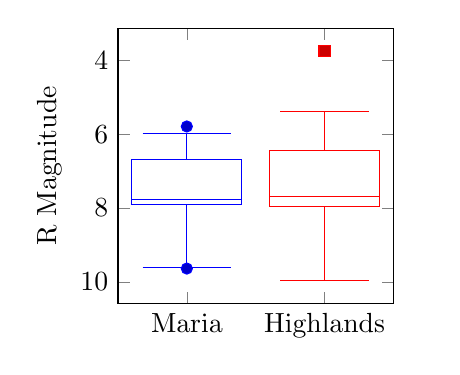
\begin{tikzpicture}
	\begin{axis}[
		width=2in,
		height=2in,
		%ylabel = R Magnitude,
		boxplot/draw direction = y,
		%boxplot/variable width,
		%boxplot={
		  %draw position={1/3 + floor(\plotnumofactualtype/2) + 1/3*mod(\plotnumofactualtype,2)},
		  %box extend = 0.3},
		%x = 4cm,
		xmin = 0.5,
		xmax = 2.5,
		xtick = {1,2,3},
		%x tick label as interval = true,
		xticklabels={ {Maria}, {Highlands} },
		x tick label style = {text width = 2.5cm, align = center},
		y label style = {align = center},
		y dir = reverse,
		ylabel = R Magnitude
	  ]
		  \addplot+[boxplot prepared={
		lower whisker = 5.97,
		lower quartile = 6.69,
		median = 7.78,
		upper quartile = 7.90,
		upper whisker = 9.61,
		sample size = 12}] coordinates {(2,5.79) (2,9.64)};

	  \addplot+[boxplot prepared={
		lower whisker = 5.38,
		lower quartile = 6.43,
		median = 7.69,
		upper quartile = 7.97,
		upper whisker = 9.97,
		sample size = 16}] coordinates {(3,3.75)};
	  
	\end{axis}
\end{tikzpicture}
\end{document}
